\chapter{Literature Review}
\label{ch:literature}

This chapter reviews the published works most related to this thesis. The chapter first describes reinforcement learning in sparse-reward environments. The next part explains why standard exploration is not enough in such settings. The chapter then reviews the main intrinsic motivation methods, including count-based and curiosity-driven exploration. Earlier work on adapting the weight of intrinsic rewards is also discussed. The chapter ends by pointing out the research gap that leads to the proposed method in Chapter 3.

\section{Reinforcement Learning in Sparse-Reward Environments}
An episodic reinforcement learning (RL) problem is commonly modeled as a Markov Decision Process (MDP) defined by the tuple $(\mathcal{S}, \mathcal{A}, P, R, \gamma, \rho_0)$, where $\mathcal{S}$ is the state space, $\mathcal{A}$ is the action space, $P(s_{t+1} \mid s_t, a_t)$ is the transition dynamics, $R$ is the reward function, $\gamma \in [0, 1)$ is the discount factor, and $\rho_0$ is the initial state distribution \cite{sutton2018rl}. At each time step $t$, the agent observes a state $s_t \in \mathcal{S}$, samples an action $a_t \sim \pi_\theta(\cdot \mid s_t)$ from a policy with parameters $\theta$, receives an extrinsic reward $R_t^E$, and moves to a new state $s_{t+1}$. This standard interaction loop is shown in Figure~\ref{fig:rl_loop}.

\begin{figure}[H]
\centering
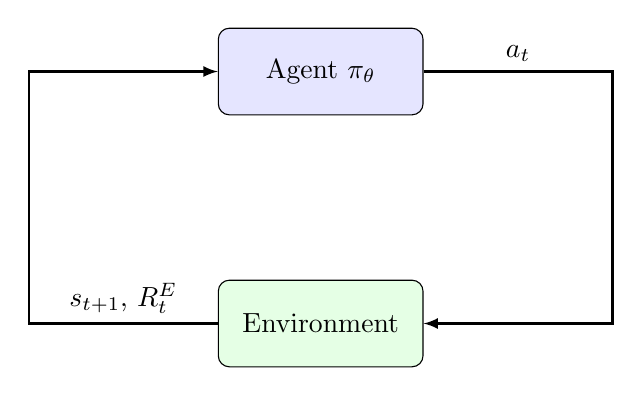
\begin{tikzpicture}[node distance=2.6cm, auto, >=latex]
    \node[draw, rectangle, rounded corners, minimum width=2.6cm, minimum height=1.1cm,
          fill=blue!10] (agent) {Agent $\pi_\theta$};
    \node[draw, rectangle, rounded corners, minimum width=2.6cm, minimum height=1.1cm,
          fill=green!10, below of=agent, node distance=3.2cm] (env) {Environment};
    \draw[->, thick] (agent.east) -- ++(2.4,0)
        node[midway, above] {$a_t$}
        |- (env.east);
    \draw[->, thick] (env.west) -- ++(-2.4,0)
        node[midway, above] {$s_{t+1}$, $R_t^E$}
        |- (agent.west);
\end{tikzpicture}
\caption{Standard agent--environment interaction loop in reinforcement learning. The agent observes a state, takes an action sampled from its policy, and receives a new state and an extrinsic reward from the environment.}
\label{fig:rl_loop}
\end{figure}

The goal of policy optimization is to learn parameters $\theta$ that maximize the expected discounted return:
\begin{equation}
J(\theta) = \mathbb{E}_{\tau \sim (\pi_\theta, P)} \left[\sum_{t=0}^{T-1} \gamma^t R_t^E \right],
\label{eq:rl_objective}
\end{equation}
where $\tau = (s_0, a_0, s_1, a_1, \dots)$ denotes a trajectory induced by the policy and the transition dynamics.

Equation~\eqref{eq:rl_objective} is a standard form. But learning becomes hard when extrinsic rewards are sparse. In sparse-reward tasks, the agent may take a long sequence of actions before getting any feedback. This feedback is needed to tell good trajectories from useless ones. Classical exploration methods such as $\epsilon$-greedy or random policies just add randomness to action choice. They do not actively guide the agent toward useful experiences when the state space is large or partly observed \cite{francois2018deep}. As a result, an agent that uses only extrinsic rewards in such environments often fails to find the goal-reaching behaviors needed to start learning.

\section{Policy Optimization Foundations}
\label{sec:policy_optimization_foundations}

This section reviews three tools that Chapter~\ref{ch:methodology} builds on: value functions and the Bellman equation, the Proximal Policy Optimization (PPO) clipped surrogate objective, and Generalized Advantage Estimation (GAE). The presentation is kept to the level of detail needed to follow Chapter~\ref{ch:methodology}.

\subsection{Value Functions and Bellman Equations}
\label{sec:value_functions}

For a policy $\pi$, the \emph{state-value function} is the expected discounted return obtained by following $\pi$ from state $s$:
\begin{equation}
V^\pi(s) \;=\; \mathbb{E}_{\pi, P}\!\left[\, \sum_{k=0}^{\infty} \gamma^k\, R_{t+k}^E \,\Big|\, s_t = s \right].
\label{eq:value_function}
\end{equation}
The \emph{action-value function} is the corresponding quantity conditioned on the next action:
\begin{equation}
Q^\pi(s, a) \;=\; \mathbb{E}_{\pi, P}\!\left[\, \sum_{k=0}^{\infty} \gamma^k\, R_{t+k}^E \,\Big|\, s_t = s,\, a_t = a \right].
\label{eq:action_value}
\end{equation}
Both functions satisfy the Bellman expectation equation \cite{sutton2018rl}:
\begin{equation}
V^\pi(s) \;=\; \mathbb{E}_{a \sim \pi(\cdot \mid s),\, s' \sim P(\cdot \mid s, a)}\!\left[\, R^E(s, a) + \gamma\, V^\pi(s') \,\right].
\label{eq:bellman}
\end{equation}
In practice, $V^\pi$ is approximated by a critic network $V_\mu$ with parameters $\mu$, trained by regression on bootstrapped targets. The critic $V_\mu$ is shared across the GAE and PPO formulas reviewed below, and reappears throughout Chapter~\ref{ch:methodology}.

\subsection{Proximal Policy Optimization}
\label{sec:ppo_background}

PPO \cite{schulman2017ppo} is the on-policy actor--critic algorithm used as the base policy optimizer throughout this thesis. Let $\pi_\theta$ be the current policy and $\pi_{\theta_\text{old}}$ the policy at the start of an update cycle. Define the importance-sampling ratio $\rho_t(\theta) = \pi_\theta(a_t \mid s_t) / \pi_{\theta_\text{old}}(a_t \mid s_t)$ and let $\hat A_t$ denote an advantage estimate. The PPO clipped surrogate objective is
\begin{equation}
L^\text{PPO}(\theta) \;=\; -\,\mathbb{E}_t\!\left[
\min\!\Bigl(
\rho_t(\theta)\, \hat A_t,\;
\text{clip}\bigl(\rho_t(\theta),\, 1 - \epsilon,\, 1 + \epsilon\bigr)\, \hat A_t
\Bigr) \right],
\label{eq:ppo_clip}
\end{equation}
where $\epsilon$ is the clipping parameter. The minimum of the unclipped and clipped terms is a pessimistic lower bound on the unclipped policy-gradient objective. This bound keeps each update inside a trust region around $\pi_{\theta_\text{old}}$. PPO alternates between collecting on-policy rollouts, fitting the critic $V_\mu$ to bootstrapped targets, and minimizing $L^\text{PPO}$ over several epochs of minibatches.

\subsection{Generalized Advantage Estimation}
\label{sec:gae_background}

GAE \cite{schulman2016gae} is the standard way to estimate $\hat A_t$ for actor--critic methods. The estimator is built from one-step temporal-difference (TD) errors of the critic:
\begin{equation}
\delta_t \;=\; R_t^E + \gamma\, V_\mu(s_{t+1})\,(1 - d_t) - V_\mu(s_t),
\label{eq:td_error}
\end{equation}
where $d_t \in \{0, 1\}$ is the episode-termination flag. GAE forms an exponentially-weighted sum of these TD errors:
\begin{equation}
\hat A_t \;=\; \sum_{l=0}^{T-1-t} (\gamma\, \lambda)^l\, \delta_{t+l},
\label{eq:gae_def}
\end{equation}
with $\lambda \in [0, 1]$ controlling the bias--variance trade-off. The limit $\lambda \to 0$ recovers the one-step TD advantage (low variance, high bias) and the limit $\lambda \to 1$ recovers the empirical Monte-Carlo advantage (high variance, low bias). Intermediate values of $\lambda$ smooth between these extremes. Equation~\eqref{eq:gae_def} is used in two places in Chapter~\ref{ch:methodology}: once with the shaped reward $\bar r_t$ for the PPO update, and once with the extrinsic-only reward $R_t^E$ for the CARE update.

With the policy optimization machinery in place, the next section turns to the intrinsic reward signals that this machinery will optimize against.

\section{Intrinsic Motivation for Exploration}
Intrinsic motivation handles sparse rewards by adding an exploration bonus on top of the environment reward. This bonus is generated by the agent itself \cite{oudeyer2007intrinsic, schmidhuber2010formal}. The standard way to formalize intrinsic motivation is to extend the MDP with an extra intrinsic reward function \cite{oudeyer2007intrinsic, schmidhuber2010formal, aubret2023intrinsic}.

\begin{definition}[Intrinsic-Augmented MDP]
\label{def:augmented_mdp}
An \emph{intrinsic-augmented MDP} is a tuple $(\mathcal{S}, \mathcal{A}, P, R^E, R^I, \gamma, \rho_0)$ in which $(\mathcal{S}, \mathcal{A}, P, R^E, \gamma, \rho_0)$ defines a standard MDP with extrinsic reward function $R^E : \mathcal{S} \times \mathcal{A} \to \mathbb{R}$, and $R^I : \mathcal{S} \times \mathcal{A} \times \mathcal{S} \to \mathbb{R}_{\ge 0}$ is an additional, internally generated intrinsic reward function. The agent observes only $(s_t, a_t, R_t^E, s_{t+1})$ from the environment; the intrinsic reward $R_t^I$ is computed by the agent itself.
\end{definition}

Under this view, the agent receives both an extrinsic reward $R_t^E$ and an intrinsic reward $R_t^I$. Policy optimization is then done on a shaped objective:
\begin{equation}
\bar{r}_t = R_t^E + \beta R_t^I,
\label{eq:shaped_reward_lit}
\end{equation}
where $\beta \ge 0$ controls how strong intrinsic motivation is. The intrinsic signal $R_t^I$ is designed to be larger for states or transitions that the agent finds new, surprising, or useful. A recent survey by Aubret \textit{et al.}~\cite{aubret2023intrinsic} brings many of these methods together under an information-theoretic view. The survey shows that intrinsic reward generators that look different can in fact be seen as different ways of applying similar core ideas.

\subsection{Count-Based Exploration}
Count-based methods give higher intrinsic rewards to states that have been visited less often. In tabular settings, the intrinsic reward at state $s$ is usually set to $1/\sqrt{N(s)}$, where $N(s)$ is the visit count. The idea is that less-explored states are more useful to revisit. Bellemare \textit{et al.}~\cite{bellemare2016count} extend this idea to high-dimensional observations through pseudo-counts from density models. Tang \textit{et al.}~\cite{tang2017exploration} use random projection hashing to get approximate counts in continuous state spaces. Ostrovski \textit{et al.}~\cite{ostrovski2017count} improve the approach with neural density models. They show strong exploration on hard Atari games such as \textit{Montezuma's Revenge}. Count-based methods are simple in idea and often work well. But the quality of the intrinsic signal is limited by how well the density estimator can measure novelty in complex observation spaces.

\subsection{Curiosity-Driven Exploration}
Curiosity-driven methods define intrinsic rewards through some form of prediction error. The Intrinsic Curiosity Module (ICM) \cite{pathak2017curiosity} learns a small latent representation of the state. ICM also trains a forward model that predicts the next latent feature from the current feature and action. The prediction error of this forward model is then used as the intrinsic bonus. This encourages the agent to seek transitions whose dynamics it cannot yet predict well. Random Network Distillation (RND) \cite{burda2019rnd} replaces the forward dynamics model with the gap between a fixed random target network and a learned predictor. This gives a state novelty signal that does not depend on action prediction. Rewarding Impact-Driven Exploration (RIDE) \cite{raileanu2020ride} computes intrinsic rewards from the size of representation changes caused by the agent's actions. This impact-based design is well suited to procedurally generated environments, where random background changes might otherwise overwhelm prediction-based bonuses.

A common benefit of curiosity-driven methods is that intrinsic rewards tend to drop as the agent becomes familiar with a region of the state space. This reduces the risk of exploring the same area again and again. However, this self-adjustment only happens at the level of the raw intrinsic signal. The weight of that signal in the shaped reward of Equation~\eqref{eq:shaped_reward_lit} is still controlled by a fixed coefficient $\beta$ that does not adapt to context.

\section{Adaptive Weighting of Intrinsic Rewards}
There are many intrinsic motivation modules, but most of them depend on a hand-tuned coefficient $\beta$ in the shaped reward of Equation~\eqref{eq:shaped_reward_lit} \cite{pathak2017curiosity, burda2019rnd}. This fixed coefficient creates a clear weakness. If $\beta$ is too small, the intrinsic signal becomes too weak and exploration stays weak. If $\beta$ is too large, curiosity may take over the training objective and distract the agent from the task. The best trade-off changes across environments and even across different stages of the same training run. So fixed weighting lacks flexibility. Several lines of research have tried to fix this weakness, with adaptation done at finer and finer levels of detail.

\subsection{Global-Level Adaptation}
A first group of methods treats the trade-off between extrinsic and intrinsic rewards as a global optimization problem. Extrinsic-Intrinsic Policy Optimization (EIPO) \cite{chen2022eipo} treats intrinsic reward weighting as an optimization with constraints. The weight of intrinsic motivation is raised only when the extrinsic objective allows it. This stops intrinsic rewards from hurting task performance. Automatic Intrinsic Reward Shaping (AIRS) \cite{yuan2023airs} treats the choice among different intrinsic reward functions as a bandit-style decision. AIRS picks which exploration signal is most useful at each phase of training. Both methods do better than hand-tuned coefficients. But their adaptation is global: a single weight or a single intrinsic reward type is chosen for the whole policy at any time, no matter what state is being visited.

\subsection{Population-Level Adaptation}
A second group of methods uses a population of policies with different exploration--exploitation trade-offs. Never Give Up (NGU) \cite{badia2020ngu} keeps several value functions tied to different intrinsic reward weights. This lets the agent share one neural network across different exploration modes. Agent57 \cite{badia2020agent57} extends this idea by also adapting the discount factor. Agent57 uses a meta-controller that picks among the population members based on their recent performance. These methods much improve robustness across many Atari benchmarks. But their adaptation works at the level of a whole policy, not at the level of single states. The shaping of intrinsic rewards inside any one policy of the population is still set by a fixed coefficient.

\subsection{Toward State-Level Adaptation}
A third and more direct line of work tries to learn the intrinsic reward signal itself. Zheng \textit{et al.}~\cite{zheng2018lirpg} propose Learning Intrinsic Rewards for Policy Gradient methods (LIRPG). A parameterized intrinsic reward function is trained via meta-gradients. The training goal is that, after a policy update using the shaped reward, the new policy maximizes the extrinsic objective. This idea is attractive because the intrinsic reward is directly tied to future extrinsic performance. In practice, however, meta-gradient training needs to differentiate through one or more policy updates. This adds a heavy computational cost and can be unstable in deep RL settings.

The research gap from this body of work is clear. Existing adaptive methods either work at a coarse level (global or population-level) or use costly higher-order optimization (LIRPG-style meta-gradients). What is missing is a lightweight mechanism that adapts the weight of intrinsic rewards at the state level. This mechanism should be trained with a first-order objective. The mechanism should also plug on top of different intrinsic reward generators without changing how they work inside.

\section{Summary and Research Gap}
This chapter has reviewed the basics on which the proposed work is built. Reinforcement learning in sparse-reward environments is hard because standard exploration methods give only weak guidance. Intrinsic motivation methods such as count-based bonuses, ICM, RND, and RIDE reduce this difficulty by adding a self-generated exploration signal. But the strength of that signal is usually set by a fixed scalar coefficient. Earlier work on adaptive weighting fixes this weakness only in part. Global and population-level methods adjust intrinsic motivation at a coarse level. Meta-gradient methods such as LIRPG work at the right level but at a high computational cost.

Two related research gaps come out of this analysis. First, there is no lightweight, state-dependent mechanism that adjusts intrinsic rewards based on how well they match future extrinsic outcomes. Yet two states with the same novelty score can contribute very differently to task success. Second, count-based bonuses, ICM, and RIDE share the same fixed-coefficient pattern. But the literature does not give a unified experimental setup that asks whether a single adaptive mechanism can improve them all in a consistent way.

The method presented in Chapter 3 is designed to fill both gaps. Chapter 3 introduces a state-dependent scaling function trained with a first-order correlation-based objective. The function works as an adaptive layer that sits above any intrinsic reward generator. The rest of the thesis builds this approach in detail and tests its effect on intrinsic reward modules in sparse-reward MiniGrid benchmarks.
